\documentclass[
	letterpaper, % Paper size, specify a4paper (A4) or letterpaper (US letter)
	10pt, % Default font size, specify 10pt, 11pt or 12pt
]{CSUniSchoolLabReport}

%----------------------------------------------------------------------------------------
%	REPORT INFORMATION
%----------------------------------------------------------------------------------------

\title{Getting Started with Linux and C++\\ Embedded Design: Enabling Robotics \\ EECE2160} % Report title

\author{Michael \textsc{Brodskiy}\\ \small \href{mailto:Brodskiy.M@Northeastern.edu}{Brodskiy.M@Northeastern.edu}}

\date{March 16, 2023} % Date of the report

%----------------------------------------------------------------------------------------


\begin{document}

\maketitle % Insert the title, author and date using the information specified above

\begin{center}
	\begin{tabular}{l r}
		Date Performed: & March 2, 2023 \\ % Date the experiment was performed
        Partner: & Dylan \textsc{Powers} \\ % Partner names
		Instructor: & Professor \textsc{Shazli} % Instructor/supervisor
	\end{tabular}
\end{center}

\newpage

\begin{abstract}

  This laboratory experiment, most importantly, served as an introduction to two main course themes: C++ programming and basic bash commands. Using this, in tandem with a secure shell connection to the De1-SoC board, rudimentary C++ code was written on the board, allowing for ease of uploading.

\end{abstract}

\begin{flushleft}

  \textsc{Keywords:} \underline{C++}, \underline{bash}, \underline{De1-SoC}

\end{flushleft}

\newpage

\section{Equipment}

\hspace{.5 in} Available equipment included:\\

\begin{itemize}

  \item DE1-SoC board

  \item DE1-SoC Power Cable

  \item USB-A to USB-B Cable

  \item Computer

  \item MobaXTerm SSH Terminal

  \item USB-to-ethernet Adapter

\end{itemize}

\section{Introduction}

\hspace{.5 in} The goal of this lab was to serve as an introduction to the DE1-SoC, an embedded computing device built around the Altera System-on-Chip (SoC) FPGA and an ARM processor, running an operating system with the GNU/Linux kernel. The lab began with the familiarization of the lab equipment and establishing a serial connection through a secure shell between the computer and the DE1-SoC board. After the connection was established, a simple \texttt{hello world} program was run on the ARM processor of the DE1-SoC. Following this program, functions to print, randomize, and sort arrays were created separately and then used in conjunction with one another. 

\section{Discussion \& Analysis} 

\subsection{Assignment 1}

The goal of Assignment 1 was to run a simple \texttt{hello world} program on the ARM processor of the DE1-SoC. The hello.cpp C++ program is displayed in the Appendix, and the output from the MobaXterm terminal is shown in Figure \ref{fig:4}. 

\begin{figure}[H]
  \centering
  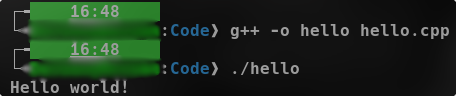
\includegraphics[width=.9\textwidth]{Figures/Assignment1.png}
  \caption{\texttt{Hello World} Program Output}
  \label{fig:4}
\end{figure}

\subsection{Assignment 2}

\hspace{.5 in} The goal of Assignment 2 was to write a more complex C++ program that generates an array of 10 random integer numbers between 0 and 99 (line 63 in source code), prints the original array (line 64 in source code), sorts the array in ascending order (line 65 in source code), and prints the sorted array (line 66 in the source code). The source code, array.cpp, is attached in the Appendix and the output on the MobaXterm terminal after the execution of array.cpp is shown in Figure \ref{fig:5}.

\begin{figure}[H]
  \centering
  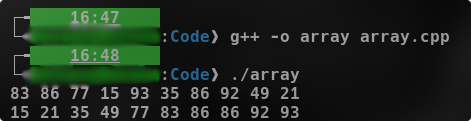
\includegraphics[width=.9\textwidth]{Figures/Assignment2.png}
  \caption{Output for Array Program}
  \label{fig:5}
\end{figure}

\subsection{Assignment 3}

\hspace{.5 in} The goal of Assignment 3 was to write a C++ program that reads in 10 random strings from the console, sorts the random strings in alphabetical order, and prints the strings sorted alphabetically. The source code, string\_sort.cpp, is included in the Appendix and the output on the MobaXterm terminal after the execution of the program is shown in Figure \ref{fig:6}.

\begin{figure}[H]
  \centering
  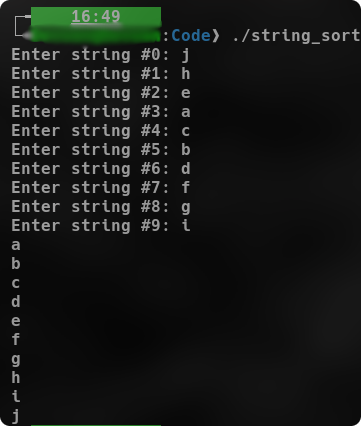
\includegraphics[width=.5\textwidth]{Figures/Assignment3.png}
  \caption{String Sort Program Output}
  \label{fig:6}
\end{figure}

\section{Conclusion}

\hspace{.5 in} Overall, this lab resulted in the creation of three C++ programs, each more complex than the list. First was a simple \texttt{Hello World} program. Next was a numerical array generator and sorter, and, finally, a string sorter. These programs allowed for a simple introduction to C++.

\section{Appendix}

\subsection{Assignment 1}

\lstinputlisting[
    caption=Hello World Source Code, % Caption above the listing
    label=lst:L1, % Label for referencing this listing
    language=C++, % Use C++ functions/syntax highlighting
    frame=single, % Frame around the code listing
    showstringspaces=false, % Don't put marks in string spaces
    numbers=left, % Line numbers on left
    numberstyle=\tiny, % Line numbers styling
    backgroundcolor=\color{black!5}, % Set background color
    keywordstyle=\color{magenta!80}, % Set keyword color
    commentstyle=\color{blue!80}, % Set comment color
    stringstyle=\color{green!80}, % Set string color
    breaklines=true
  ]{Code/hello.cpp}

  \subsection{Assignment 2}

\lstinputlisting[
    caption=Array Generator Source Code, % Caption above the listing
    label=lst:L2, % Label for referencing this listing
    language=C++, % Use C++ functions/syntax highlighting
    frame=single, % Frame around the code listing
    showstringspaces=false, % Don't put marks in string spaces
    numbers=left, % Line numbers on left
    numberstyle=\tiny, % Line numbers styling
    backgroundcolor=\color{black!5}, % Set background color
    keywordstyle=\color{magenta!80}, % Set keyword color
    commentstyle=\color{blue!80}, % Set comment color
    stringstyle=\color{green!80}, % Set string color
    breaklines=true
  ]{Code/array.cpp}

  \subsection{Assignment 3}

\lstinputlisting[
    caption=String Sorter Source Code, % Caption above the listing
    label=lst:L3, % Label for referencing this listing
    language=C++, % Use C++ functions/syntax highlighting
    frame=single, % Frame around the code listing
    showstringspaces=false, % Don't put marks in string spaces
    numbers=left, % Line numbers on left
    numberstyle=\tiny, % Line numbers styling
    backgroundcolor=\color{black!5}, % Set background color
    keywordstyle=\color{magenta!80}, % Set keyword color
    commentstyle=\color{blue!80}, % Set comment color
    stringstyle=\color{green!80}, % Set string color
    breaklines=true
  ]{Code/string_sort.cpp}

\end{document}
